\section{Experiments} \label{sec:experiment}
In this section, we measure the overall performance of the optimized 
OpenCL based BFS accelerator on Intel Xeon-FPGA, a closely coupled CPU-FPGA
architecture, over a set of representative graphs. Then we compare the 
resulting accelerator to the reference design in an HLS benchmark Spector 
as well as prior hand crafted design. Finally, we also analyze the 
graph reordering and batching comprehensively.

\subsection{Experiment Setup}
The graph benchmark used in this work includes three real-world graphs and 
two synthetic graphs generated using R-MAT model \cite{chakrabarti2004rmat} 
as listed in Table \ref{tab:graph}. The real-world graphs are from social network \cite{yang2012defining, 
leskovec2009community, takac2012data} while the R-MAT graphs are generated 
using the Graph 500 benchmark parameters ($A=0.59, B=0.19, C=0.19$). To make the 
presentation easier, the five benchmark graphs are shorted as YT, 
LJ, Pokec, R-MAT\uppercase\expandafter{\romannumeral1}, 
R-MAT\uppercase\expandafter{\romannumeral2} respectively. We refer 
to an R-MAT graph with scale $S$ ($2^{S}$ nodes) and edge factor $E$ ($E\times 2^{S}$). 
In the experiments, we averaged 64 BFS with random starting points. 
In order to avoid trivial search, we remove the BFS with less than 3 levels.

\begin{table}
    \centering
  \caption{Graph Benchmark}
  \label{tab:graph}
  \begin{tabular}{cccc}
    \toprule
      Name & \# of vertex & \# of edge & Type \\
    \midrule
      YT \cite{yang2012defining} & 1157828 & 2987624 & Undirectional \\
      LJ \cite{leskovec2009community} & 4847571 & 68993773 & Directional \\
      PK \cite{takac2012data} & 1632804 & 30622564 & Directional \\
      R-MAT\uppercase\expandafter{\romannumeral1} & 524288 & 16777216 & Directional \\
      R-MAT\uppercase\expandafter{\romannumeral2} & 2097152 & 67108864 & Directional \\
  \bottomrule
\end{tabular}
\vspace{-1em}
\end{table}

\subsection{Performance evaluation}
\subsubsection{Overall performance}
We use million traverse per second (MTEPS) as 
the performance metric. The performance of the proposed BFS 
accelerator on the graph benchmark is 
presented in Table \ref{tab:performance-summary}. 
It achieves up to 934.2 MTEPS on the R-MAT\uppercase\expandafter{\romannumeral2}
and 557.8 MTEPS on average. When compared to the reference BFS 
implementation in Spector, the proposed design shows 6.6X and 12.3X 
speedup on YT graph and R-MAT\uppercase\expandafter{\romannumeral1} 
graph respectively while Spector fails on the other three graphs with larger data sets 
because of bugs in the code. In general, the proposed design performs better on 
R-MAT graphs with higher average degree. On the contrast, YT with 
low average degree suffers higher reordering and batching cost. In addition, 
YT is an undirectional graph while the accelerator takes each edge as bidirectional ones. 
Therefore, this also leads to relatively lower MTEPS in the experiments. 
\begin{table}
    \centering
  \caption{Performance summary}
  \label{tab:performance-summary}
  \begin{tabular}{cccccc}
    \toprule
      Benchmark & YT & LJ & Pokec & R-MAT\uppercase\expandafter{\romannumeral1} & R-MAT\uppercase\expandafter{\romannumeral2} \\
    \midrule
      MTEPS & 79.4 & 475.7 & 557.8 & 787.7 & 934.2 \\
      Speedup & 6.6X & - & - & 12.3X & - \\
  \bottomrule
\end{tabular}
\vspace{-1em}
\end{table}

%The proposed design needs a coupled CPU to reorganize the RPA based on the frontier vertices.
%The process has a lot of random access and it is appropriate for CPU because 
%of the optimized cache sub system. To evaluate the approach, we further analyze the 
%execution time distribution of the BFS. According to Figure \ref{fig:runtime}, the CPU execution time 
%takes a small proportion of the whole execution time in general, while the proportion is relatively 
%higher for the social network graphs which have deeper levels and more processing on CPU 
%compared to the R-MAT graphs. 
%\begin{figure}
%	\center{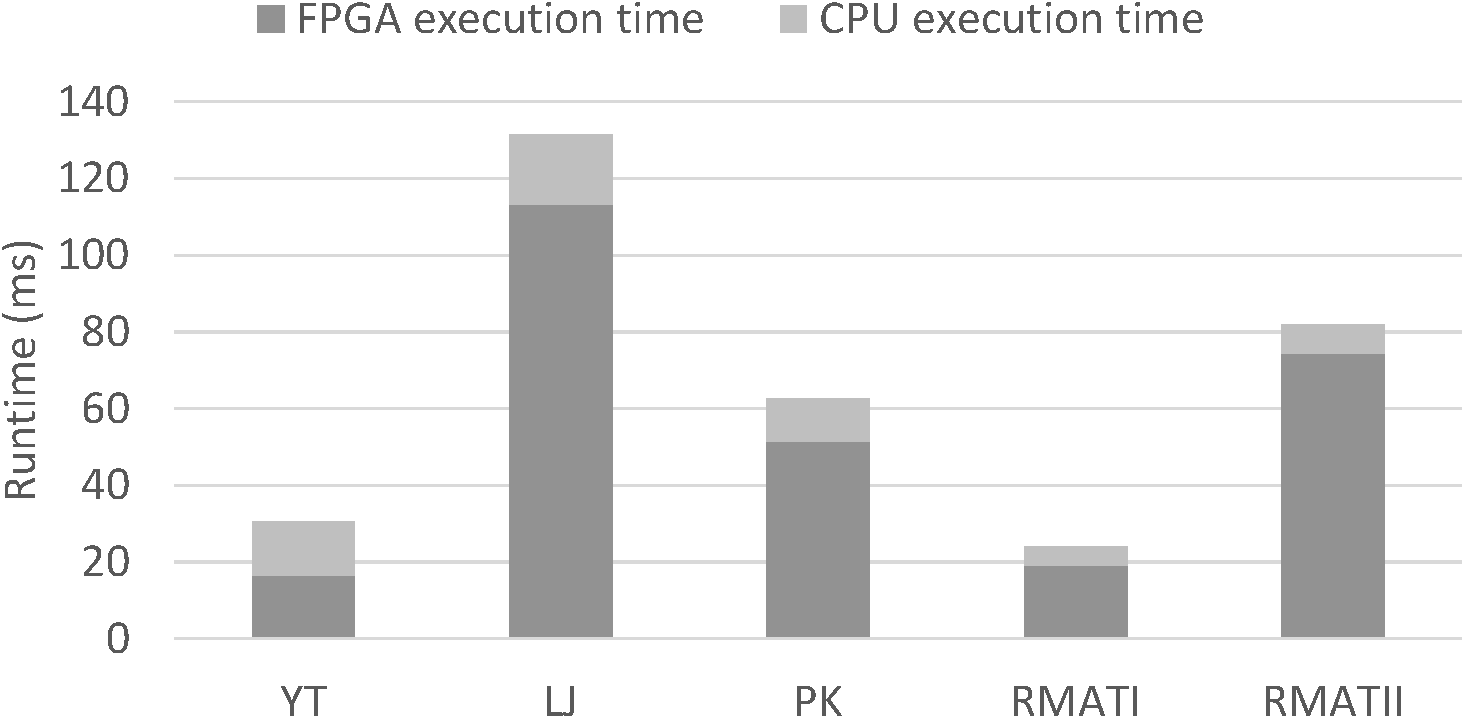
\includegraphics[width=0.85\linewidth]{runtime}}
%    \caption{Runtime distribution of the BFS accelerator on different graphs}
%\label{fig:runtime}
%\vspace{-1em}
%\end{figure}

\subsubsection{Performance comparison}
On top of the comparison to the reference OpenCL design, we also compare 
this work to prior published BFS accelerators on FPGAs. As the platforms 
and graph benchmark used in these work are mostly different, it is 
difficult to make a completely fair end-to-end comparison. 
A summary of prior FPGA based BFS acceleration work is presented in Table \ref{tab:compare}. 
It can be found that the OpenCL based BFS accelerator proposed in this work achieves 
comparable performance to many prior hand crafted design and even outperforms some of them 
particularly on R-MAT graphs. When compared to design on high-end 
FPGA computing system with multiple FPGAs like Convey HC2\cite{attia2014cygraph}, 
the overall performance in this work is still lower, 
but the performance per FPGA is better. In addition, the OpenCL based design 
gains the software-like features and can be easily ported to similar FPGA boards.
Note that 'S' in the last column of the table indicates that the performance is obtained by simulation. 
Accordingly, 'M' means that the performance is measured based on hardware implementation. 

\begin{table}
  \caption{FPGA based BFS accelerator performance comparison}
  \label{tab:compare}
    \setlength{\tabcolsep}{4pt} % Default value: 6pt
    %\renewcommand{\arraystretch}{1.5} % Default value: 1
  \begin{tabular}{ccccc}
    \toprule
	Year & System & Platform & MTEPS/FPGA & Method\\
    \midrule
	2010 & Qingbo's work \cite{wang2010message} & Virtex-5 & 160-790 & S \\
	2012 & Betkaouis'work\cite{betkaoui2012reconfigurable} & Convey HC-2 & 62.5-650 & M \\
	2014 & CyGraph\cite{attia2014cygraph} & Convey HC-2    & 420-550 & M \\
	2015 & Umuroglu's work\cite{umuroglu2015hybrid} & Zedboard & 90-255 & M \\
	2016 & FPGP\cite{dai2016fpgp} & VC707 & 122 & M\\
	2016 & GraVF\cite{engelhardt2016gravf} & Virtex-7 & 3500 & M \\
	2017 & ForeGraph\cite{Dai2017foregraph} & VCU110 & 364-1069 & S\\
	2017 & Jialiang's work\cite{zhang2017boosting} & AC-510 & 130-166 & M/S\\
	2017 & Shijie's work \cite{zhou2017accelerating} & Harp-v1 & 330 - 670 & M\\
	2018 & Jialiang's work \cite{zhang2018degree} & AC-510 & 400-1526 & M/S \\
	2018 & Soroosh's work \cite{khoram2018accelerating} & AC-510 & 100-650 & M \\
	2018 & Pengcheng's work\cite{yao2018efficient} & Ultrascale+ & 1500-3500 & S \\
	2018 & GraFBoot\cite{jun2018grafboost} & VC707+Flash & 57-75 & M \\
	\midrule
	2019 & OBFS (R-MAT Graph) & Harpv2 &  861 & M\\
	2019 & OBFS (Social Network) & Harpv2 & 371 & M\\
  \bottomrule
\end{tabular}
\vspace{-1em}
\end{table}

\subsubsection{Optimization approach analysis}
As mentioned, we mainly apply three different approaches including 
graph reordering, on-chip buffer partition,  
and hype pipelining to optimize the OpenCL based BFS accelerator.
While the graph reordering and on-chip buffer partition are naturally combined, 
we have the two optimizations evaluated together. The performance improvement 
by gradually applying the optimizations to the BFS accelerator is presented 
in Figure \ref{fig:opt-analysis}. Note that the accelerators with different 
optimizations have 8Mb bitmap implemented. Batch size is set to be 16.
It can be found that the graph reordering and on-chip buffer partition 
contributes most to the overall performance improvement. 
4X - 14X speedup over the base design is achieved on the graph benchmark. 
Hyper pipelining is also demonstrated to be beneficial. 
It improves the performance by 9.8\% to 16.7\%. 

 \begin{figure}
	\center{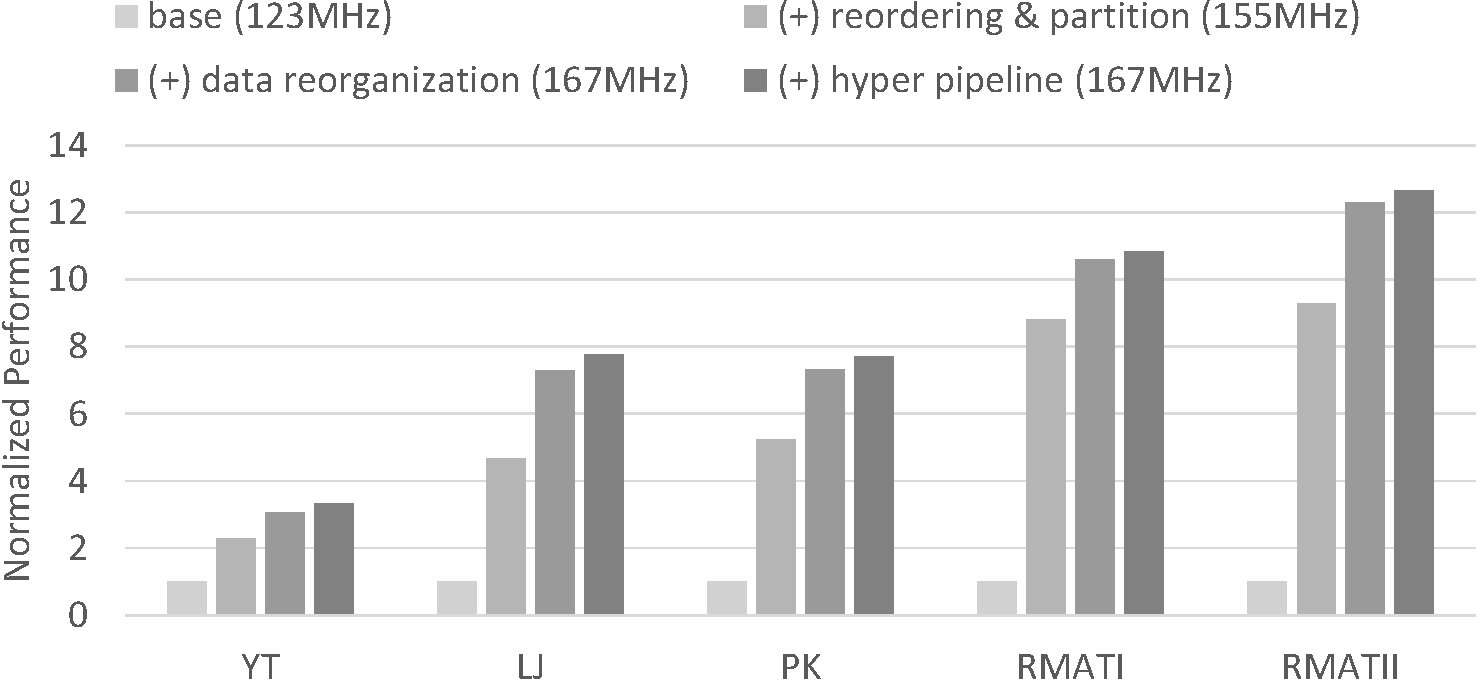
\includegraphics[width=0.85\linewidth]{opt-analysis}}
	\caption{Performance improvement with different high-level optimizations}
\label{fig:opt-analysis}
\vspace{-1em}
\end{figure}

When different optimizations are applied to the OpenCL based BFS accelerator, 
the resulting FPGA implementation frequency is also different. 
Particularly, LJ has more than 4 million vertices and we set the bitmap buffer to be 8Mb. 
For the rest of the graphs with less than 4 million vertices, we set the bitmap to be 4Mb. 
Table \ref{tab:opt-freq} shows the resulting accelerator frequency. 
It can be found that the proposed OBFS produces higher hardware 
implementation frequency which also contributes to the resulting 
performance improvement. 

\begin{table}
  \caption{Implementation frequency of the BFS with different high-level optimizations}
  \label{tab:opt-freq}
    \setlength{\tabcolsep}{4pt} % Default value: 6pt
    %\renewcommand{\arraystretch}{1.5} % Default value: 1
	\centering
  \begin{tabular}{cccc}
    \toprule
	bitmap & base & (+) reordering\&partition & hyper pipelining \\
	\midrule
	4Mb & 123 MHz & 155 MHz & 202 MHz\\
	8Mb & 110 MHz & 142 MHz & 165 MHz\\
  \bottomrule
\end{tabular}
\vspace{-1em}
\end{table}


\subsection{Batch trade-offs}
Graph reordering and batching contributes most to the BFS performance 
improvement and will be analyzed in this subsection. 
Figure \ref{fig:batch-perf} shows the BFS performance of different batch size.
In general, larger batch size induces higher performance and batch 16 
achieves the best performance on all the benchmark graphs. BFS performance 
starts to drop when the batch size is larger.  
\begin{figure}
	\center{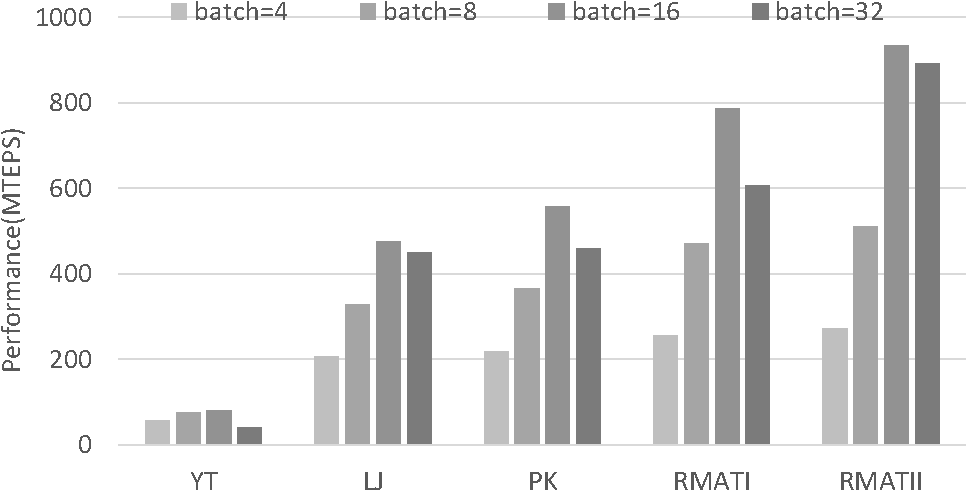
\includegraphics[width=0.8\linewidth]{batch-perf}}
    \caption{BFS performance of different batch size}
\label{fig:batch-perf}
\vspace{-1em}
\end{figure}


The proposed graph reordering and batching approach expands the 
graph layout and it will induce more memory overhead. The batch overhead 
on the benchmark graphs is illustrated in Figure \ref{fig:batch-overhead}. 
When the batch size increases, the CSR data increases accordingly. 
Particularly, it can be seen that data replication overhead 
increases dramatically when the batch size reaches 32. 
As a result, the performance benefit is compensated 
by the additional data replication and memory access.
While YT has the lowest average degree, it has the least performance 
speedup with larger batch size and drops dramatically at batch 32.

\begin{figure}
	\center{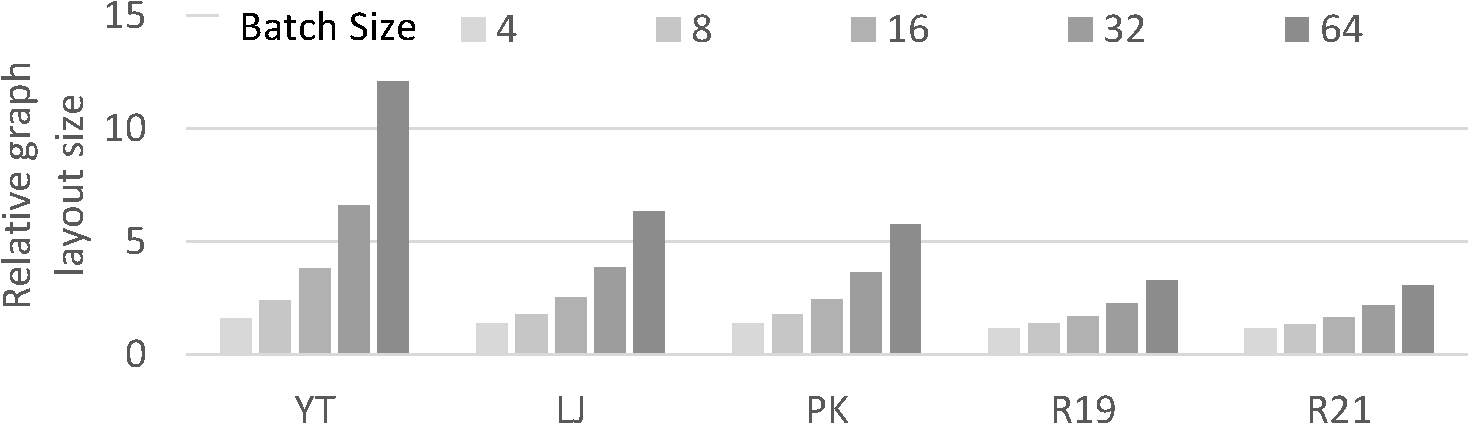
\includegraphics[width=0.85\linewidth]{batch-overhead}}
    \caption{Relative memory overhead of different batch size}
\label{fig:batch-overhead}
\vspace{-1em}
\end{figure}

The advantages of the batch are multi-folded.
In particular, batch mainly has the memory 
access coalesced and improves the memory bandwidth utilization, 
In combination with the bitmap, the irregular memory access 
reduces by more than 90\% compared to the base design.
As experimented in Section \ref{sec:motivation}, batched memory 
access has much lower average memory access latency and thus memory 
bandwidth utilization. In general, to trade-off the batch 
overhead and the performance benefit, 
larger batch size is recommended for graphs with higher average degree 
and smaller batch size is better for graphs with lower degree 
such as YT.  


%For sequential memory access and random access, 
%we performed independent experiments on Harp-v2 
%to evaluate the benefits. We measured the transfer time 
%of 64MB data in different batch size and calculated the 
%corresponding bandwidth. The bandwidth is normalized to 
%the transfer with 32-bit data width. The relative bandwidth result is presented in 
%Figure \ref{fig:mem-bandwidth}. Note that dependent random access pattern 
%refers to the random accesses that can only proceed one after another.
%This happens in the OpenCL based BFS. As low-degree frontier 
%vertices in each data path traverse sequentially because the compiler 
%has no clue if there is data dependency between different frontier 
%neighbors. 
%
%\begin{figure}
%	\center{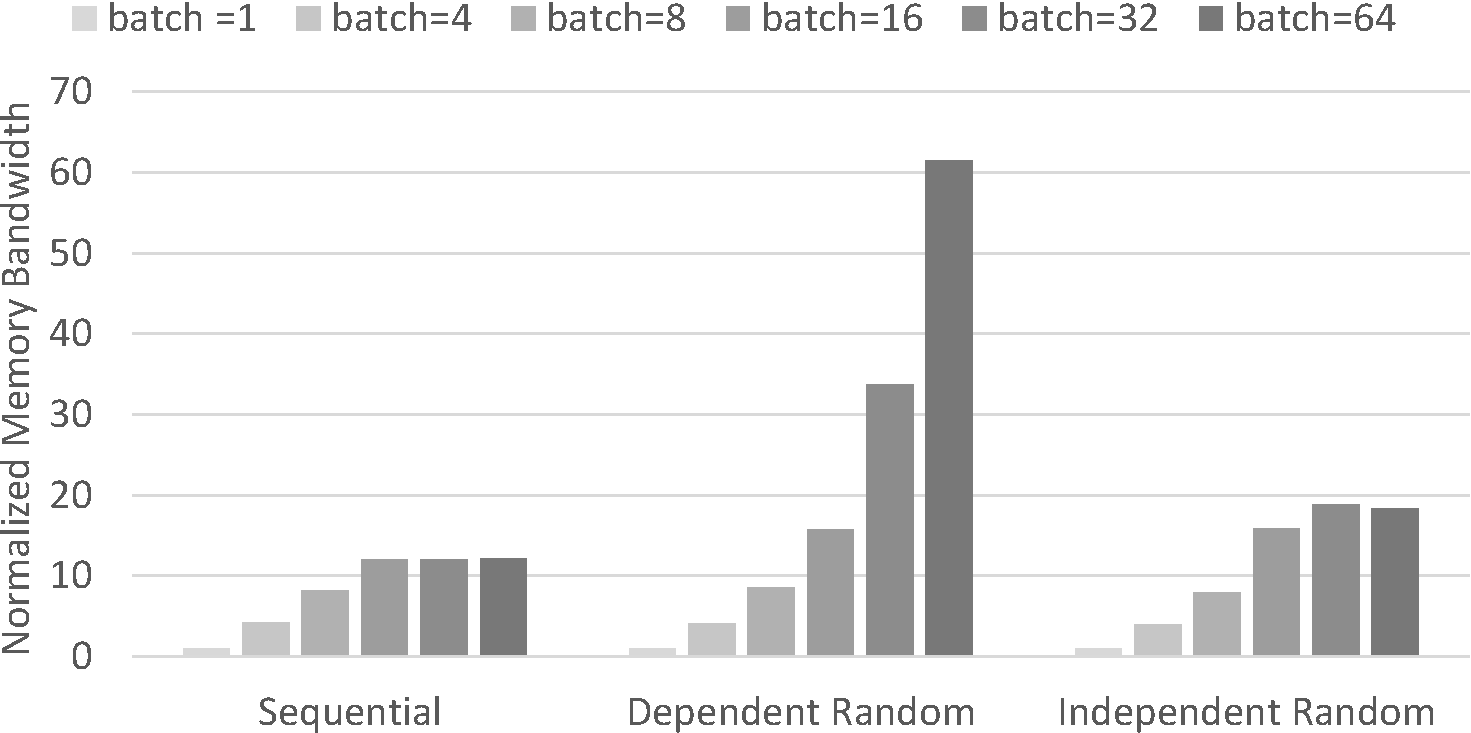
\includegraphics[width=0.85\linewidth]{mem-bandwidth}}
%    \caption{Batch size influence on memory bandwidth}
%\label{fig:mem-bandwidth}
%\vspace{-1em}
%\end{figure}


%It is clear that the bandwidth utilization of batched random memory access
%improvement is significantly higher than that of the sequential memory access. 
%Particularly, dependent random memory access keeps continuous memory 
%bandwidth utilization improvement when the batch size goes up to 64,
%While the independent random memory access gets saturated when 
%the batch size reaches to 32. It indicates that the OpenCL tools 
%can actually explore memory level parallelism of random memory access.
%For sequential memory access, the bandwidth utilization saturates 
%when the batch size is 16 and the data width equals to the 
%internal 512 bit. In general, the experiment exhibits the potential 
%memory bandwidth utilization improvement of BFS using the proposed 
%reordering and batching.

\subsection{Hardware implementation}
\subsubsection{Resource overhead}
The FPGA resource consumption and the implementation frequency of 
the proposed accelerator with different configurations 
is listed in Table \ref{tab:resource}. 

According to the table, Harp-v2 platform already consumes 
a large portion of the FPGA resources while the BFS accelerator resource 
consumption is moderate. Particularly, the memory blocks consumption of 
16Mb BFS accelerator actually takes around 47\% of the total FPGA 
RAM blocks. The total on-chip FPGA buffer allows at most 32 Mb bitmap 
to be implemented. It is the resource bottleneck of the BFS 
accelerator for larger bitmap or graphs with more vertices.

Larger batch size ensures more parallel BFS data paths and 
more logic resources will be required as shown in 
Table \ref{tab:resource}. In addition, more 
parallel memory access ports in the BFS accelerator also lead to 
slightly more block RAM overhead which is implicitly generated by the Intel 
OpenCL compiler. This can also be observed from the table.

\begin{table}
  \caption{FPGA resource consumption with different configurations}
  \label{tab:resource}
  %\setlength{\tabcolsep}{4pt} % Default value: 6pt
  %\renewcommand{\arraystretch}{1.5} % Default value: 1
    \centering
  \begin{tabular}{cccc}
    \toprule
	\shortstack{Config. \\ (batch, bitmap)} & \shortstack{Logic \\ Resource} & \shortstack{RAM \\ blcoks} & \shortstack{Frequency \\ (MHz)} \\
	\midrule
	  bare platform   & 24\% & 8\%  & -   \\
	  \midrule
	  (4, 4Mb)   & 29\% & 26\% & 158 \\
	  (8, 4Mb)   & 32\% & 27\% & 172 \\
	  (16, 4Mb)  & 37\% & 28\% & 201 \\
	  (32, 4Mb)  & 49\% & 29\% & 208 \\
	  \midrule
	  (4, 8Mb)  & 28\% & 36\% & 144 \\
	  (8, 8Mb)  & 31\% & 36\% & 153 \\
	  (16, 8Mb) & 37\% & 38\% & 165 \\
	  (32, 8Mb) & 48\% & 40\% & 177 \\
	  \midrule
	  (4, 16Mb)  & 28\% & 55\% & 132 \\
	  (8, 16Mb)  & 31\% & 55\% & 128 \\
	  (16, 16Mb) & 37\% & 57\% & 148 \\
	  (32, 16Mb) & 48\% & 59\% & 149 \\
	  \midrule
      Spector    & 39\% & 36\% & 190 \\
  \bottomrule
\end{tabular}
\vspace{-1em}
\end{table}

\subsubsection{Implementation frequency}
In Table \ref{tab:resource}, we show the BFS accelerator implementation frequency.
The proposed BFS accelerator can reach 208 MHz when the bitmap is 4Mb and batch is 32.
Typically, larger batch size which essentially indicates smaller bitmap partitions
is more friendly to the placing and routing and beneficial to the hardware implementation 
eventually. Accordingly, the implementation frequency of the BFS accelerator increases. 
While bitmap size has negative influence on the hardware implementation frequency
and higher frequency promises higher performance, we will choose the BFS 
accelerator with highest implementation frequency when the graph can be fit into 
the bitmap.

